\documentclass[a4paper,10pt]{beamer}
\usepackage[utf8x]{inputenc}
\usepackage[T1]{fontenc}
\usepackage[english]{babel}
\usepackage{hyperref,graphicx}
\usetheme{Berkeley}

\setbeamertemplate{navigation symbols}{\insertframenumber /\inserttotalframenumber}

\title{3D object from a 2D drawing}
\author[Groupe 3INFO]{Aurélien Fontaine, Manutea Huang, Etienne Geantet, Arnaud Martin}
\institute[INSA de Rennes]{Institut National des Sciences Appliquées de Rennes}
\date{\today}

\begin{document}
	\begin{frame}
		\begin{titlepage}
			\centerline{
\includegraphics[scale=0.1]{images/logoINSA.jpg}}
			Encadrants : François Lehericey	et Bertrand	Coüasnon	
		\end{titlepage}
	\end{frame}
	
	\begin{frame}
		\tableofcontents
	\end{frame}
	
	\section{Introduction}
	
		\subsection{Our subject}
	
			\begin{frame}{The subject}
				\begin{itemize}
					\item Create an object from a drawing on a tablet
					\item An easy use, the creation in less than a minute
				\end{itemize}
				Final objective : Occupy a room with simple objects made by an user
			\end{frame}
			
		\subsection{Existing technologies}
			
			\begin{frame}{A project made by Sony}
				Project PS4 : The PlayRoom (actually available)
				\href{run:The_PlayRoom.avi}{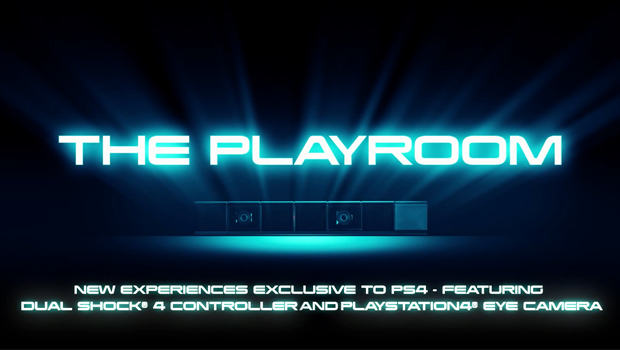
\includegraphics[width=300pt]{images/The-Playroom.jpg}}
			\end{frame}
			
			\begin{frame}{Drawing editors}
				\begin{itemize}
					\item A lot of drawing editors : Markers, LayerPaint, SketchBook, ...
					\item Great drawings
					\item No possibility of making a 3D object
					\item Source code inaccessible
				\end{itemize}
			\end{frame}
	
	\section{Our graphic solution}
		\subsection{Specifications}
		
		\begin{frame}{Specifications}
			\begin{itemize}
				\item An ergonomic application
				\item A tablet application
				\item The exportation have to be compatible with Unity
				\item Create 3D objects more or less complex (simple balloon, or a car with its wheels)
			\end{itemize}
		\end{frame}
		
		\subsection{The interface}
		
			\begin{frame}{The app}
				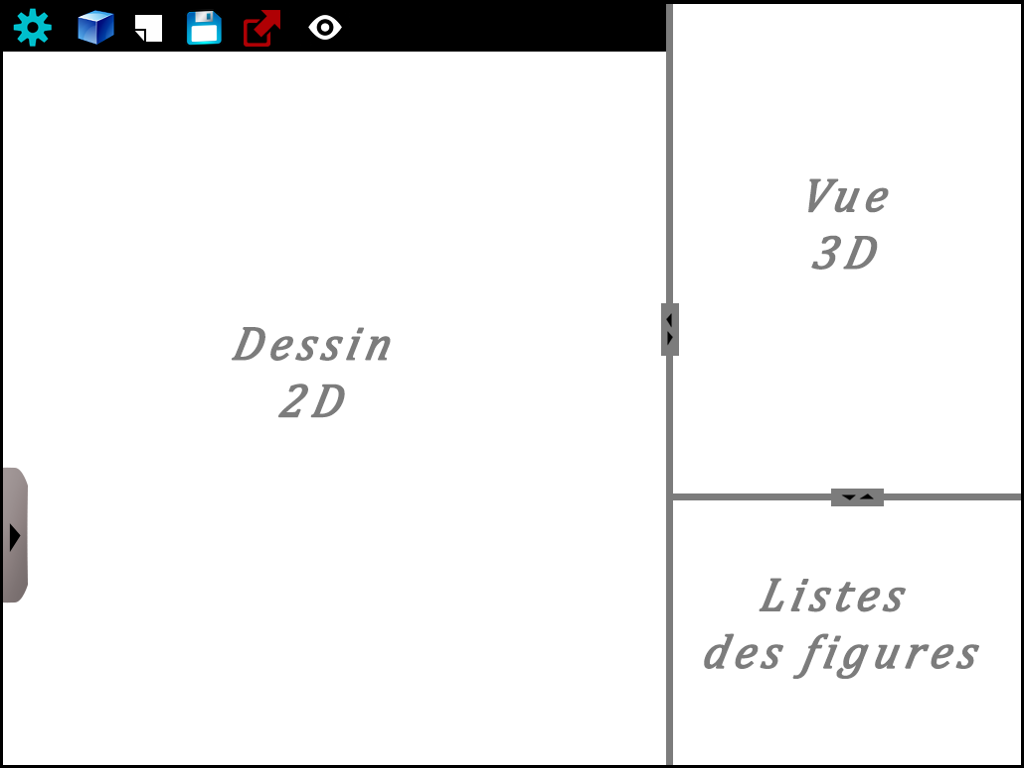
\includegraphics[height=205pt]{images/AppliMenuFerme.png}
			\end{frame}
			
			\begin{frame}{The app}
				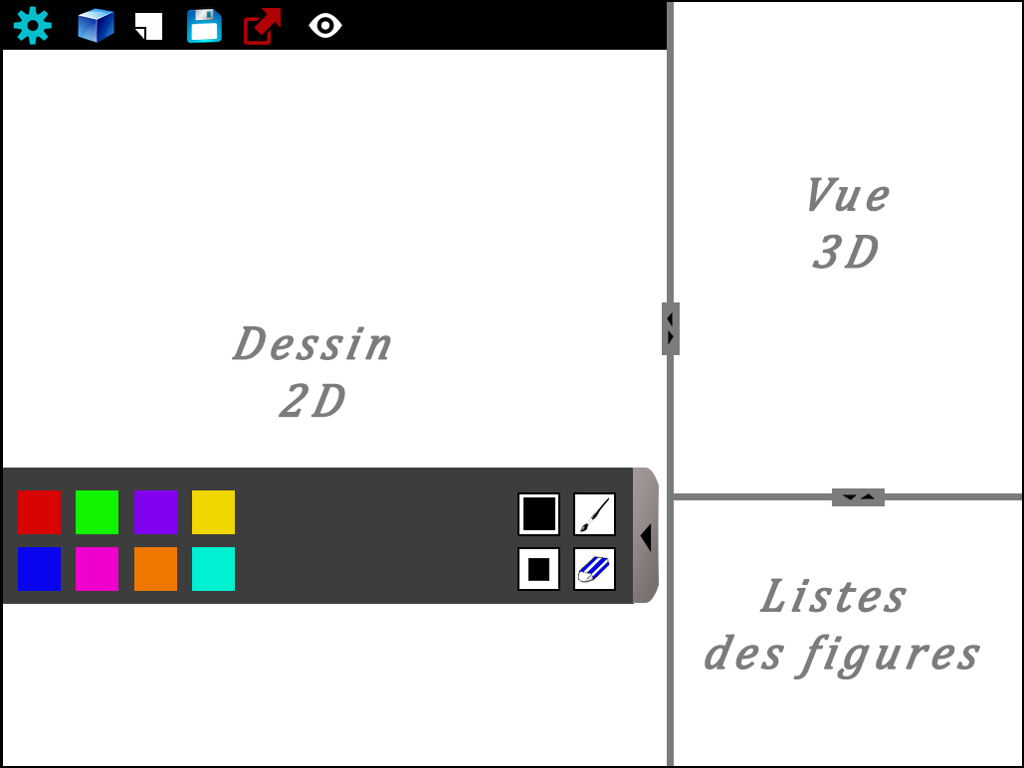
\includegraphics[height=205pt]{images/AppliMenuOuvert.png}
			\end{frame}
			
		\subsection{The tools}
		
			\begin{frame}{User's possibilities}
				A voir si vraiment utile ...
				
				If the user press the save button(
\includegraphics[height=10pt]{images/saveIcone.png}), the project will be save.
			\end{frame}
	
	\section{The technology : the engines}
	
		\subsection{Unity}
		
			\begin{frame}{Unity}
				
\includegraphics[height=75pt]{images/Logo_Unity.jpg}
				
				 An IDE tool-kit with assets, basically a framework. 
			\end{frame}
			
		\subsection{FPS game-engine}
		
			\begin{frame}{Unreal Engine}
				
\includegraphics[height=120pt]{images/Unreal_Engine.png}\\
				A game engine made for FPS
				\begin{itemize}
					\item Few help to develop on tablets
					\item Have to go around for simple tasks (the interface = a pause menu)
				\end{itemize}
			\end{frame}
			
			\begin{frame}{CryEngine}
				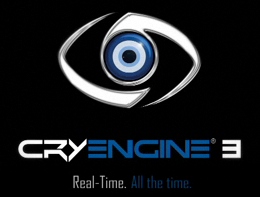
\includegraphics[height=100pt]{images/Cry_Engine.png}
			\end{frame}
			
		\subsection{Others}
			
			\begin{frame}{OpenGl}
				
\includegraphics[height=75pt]{images/OpenGL_logo.png}
				\begin{itemize}
					\item A language hardware oriented (hard to change of devices)
					\item A long time to learn how to use it
					\item A lot of code lines just for a simple form
				\end{itemize}
			\end{frame}
			
			\begin{frame}{Autodesk Maya}
				\includegraphics[height=75pt]{images/AutoDesk_Maya.png}
			\end{frame}
			
	\section{Conclusion}
		
		\begin{frame}{Conclusion}
			We have chosen Unity for multiple reasons :
			\begin{itemize}
				\item Easy to use on different OS
				\item An engine very powerful with a few lines
				\item The exportation between two devices under Unity is simple
			\end{itemize}			
		\end{frame}
	
\end{document}
